\chapter{Teoria dei grafi e delle reti sociali}

\section{Esperimento di Granovatter}

Nel 1960, il sociologo Mark Granovetter effettuò il seguente esperimento nella sua tesi di dottorato: intervistò una serie di persone che di recente avevano cambiato lavoro, facendo domande poste a capire in che modo erano venuti a conoscenza della nuova opportunità lavorativa.

Come ci si può aspettare la gran parte delle persone erano venuti a conoscenza dell'opportunità da lavoro tramite passaparola.

Ciò che invece era meno atteso, è che un gran numero di volte l'informazione arrivò da gente che si conosceva superficialmente.
Questo fu sorprendente perché ci si aspetta che gli amici più stretti siano quelli più interessati ad aiutarsi nel momento del bisogno.

Una risposta al fenomeno proposta da Granovetter fu che le persone a noi strette in realtà tendono ad avere le stesse nostre informazioni.
Infatti è normale che se frequentino più o meno gli stessi posti e persone di un amico stretto.
Oppure, se ho una relazione stretta con una persona è perché ci ho parlato molto nel tempo, e quindi tutte le informazioni importanti che tale persona poteva darmi me le avrà già date in passato.

Contrariamente, una persona che conosco poco probabilmente frequenterà altri posti e persone, e quindi avrà accesso ad altre fonti di informazioni che provengono al di fuori della mia comunità.

\subsection{Bridge \& Local Bridges}

Consideriamo il grafo $G = (V, E)$ che modella la rete, gli archi che "aumentano" le nostre informazioni sono quelli che ci collegano a regioni della rete \textit{inaccessibili} ai nostri amici.

\begin{definizione}[Bridge]
    Definiamo un \textbf{bridge} come un arco la cui rimozione rende la rete disconnessa. Dall'esperimento di Granovatter, segue che i bridge sono gli archi che hanno maggione "valore informativo".
\end{definizione}

In una rete sociale reale (e artificiale) è davvero molto poco probabile che esistano bridge edges, anche perché sappiamo già che le reti sociali presentano delle componenti giganti con buona probabilità. Dobbiamo quindi rilassare le definizione di bridge.

\begin{definizione}[Local Bridge]
    Definiamo \textbf{local bridge} un arco $(u,v)$ se $u$ e $v$ non hanno altri amici in comuni, ovvero se $N(u) \cup N(v) \equiv \emptyset$
    
    Possiamo vedere i local bridge come archi la cui rimozione aumenta la distanza tra le due estremità di almeno 2.
\end{definizione}

\subsection{Weak \& Strong Ties}

Dall'esperimento di Granovatter, oltre a identificare il potere "informativo" degli archi, mostra anche che l'informazione arriva da qualcuno conosciuto solo superficialmente, e non dagli amici stretti. Possiamo quindi identificare due tipologie di relazioni: 
\begin{itemize}
    \item \textbf{Relazione Forte (Strong Tie)}: sono quelle relazioni che ci collegano agli amici stretti.
    \item \textbf{Relazione Debole (Weak Tie)}: sono quelle relazioni che ci collegano ai semplici conoscenti.
\end{itemize}
Di conseguenza, possiamo modellare una rete di questo tipo mediano un grafo $G$, in cui gli archi sono partizionati in due sottoinsiemi:
\[
G = (V, S \cup W) \text{ con } S \cap W = \emptyset
\]
E come ha mostrato l'esperimento di Granovatter, gli archi deboli veicolano informazioni alle quali non avremmo accesso tramite gli archi forti, e questa è la \textbf{forza degli archi deboli}.

\subsection{Strong Triadic Closure Property}

Consideriamo lo stato di una rete sociale in un dato istante, sarebbe interessante sapere come si evolve nel tempo e quali sono i meccanismi che portano alla creazione o alla rottura di nuovi archi.

Un principio abbastanza intuitivo è il seguente: se due nodi hanno un amico stretto in comune, allora è molto probabile che in futuro entrino in contatto e stabiliscano anch'essi un rapporto di amicizia stretta. Ciò che si genera quindi tra i tre nodi in questione è la cosiddetta \textbf{chiusura triadica}.

Pensando la chiusura triadica in termini di strong e weak ties possiamo definirla secondo la seguente regola:
\begin{definizione}[Chiusura Triadica]
Sia il nodo $a$ e due suoi vicini $b$ e $c$, allora l'arco $(b,c)$ probabilmente si creerà se $(a,b),\ (a,c) \in S$, ovvero se sono una \textbf{strong tie}.
\end{definizione}

\begin{definizione}[Strong Triadic Closure Property (STCP)]
Sia $G = (V, S\cup W)$; un nodo $u$ soddisfa la \textbf{proprietà della chiusura triadica forte} se, per ogni coppia di archi incidenti su $u$, i loro estremi sono collegati da un arco. Formalmente:
\[
u \in V \text{ soddisfa la STCP } \iff \forall(u, v),(u, w) \in S: [(v, w) \in S \cup W]
\]
$G$ soddisfa la STCP se tutti i nodi la soddisfano.
\end{definizione}
Se si osserva bene, quando una rete soddisfa la STCP essa si \textbf{stabilizza} secondo la regola precedentemente descritta, ovvero in futuro non si genereranno più altri archi.

\subsection{STCP \& Local Bridges}

\begin{teorema}
    Sia $G=(V, S \cup W)$; se un nodo $u \in V$ soddisfa la STCP e se esistono due nodi distinti $x$ e $z$ tali che $(u, x) \in S$ e $(u, z)$ è un local bridge (ovvero $N(u) \cap N(z) = \emptyset$), allora $(u,z) \in W$, ovvero è un weak tie (arco debole).
\end{teorema}
\begin{proof}
    Poiché $(u,z)$ è un local bridge, allora $N(u) \cap N(z) = \emptyset$ (per definizione di local bridge). Se per assurdo $(u, z) \in S$, allora, poiché $(u,x) \in S$ e $u$ soddisfa la STCP, dovrebbe esistere l'arco $(x, z) \in S \cup W$, ossia sarebbe che che $x \in N(u) \cap N(z)$ che per ipotesi è uguale all'insieme vuoto - \textbf{Assurdo!}
\end{proof}

Questo teorema mostra come \textit{una proprietà globale (essere un local bridge) si riflette in una proprietà locale (essre un weak tie)}. Infratti:
\begin{itemize}
    \item Essere weak tie è proprietà locale: un nodo sa da solo se un suo vicino è un amico o un conoscente.
    \item Essere local bridge è una proprietà globale: un nodo deve chiedere a tutti i suoi vicini se qualcuno di loro conosce un suo conoscente per sapere se è un local bridge.
\end{itemize}

Infatti, nell'esperimento di Granovetter, i weak ties, in quanto portatori di informazioni erano anche local bridges.

\subsection{Comunità e Coefficiente di Clustering}

Abbiamo definito in precedenza un modello di rete dinamica i cui archi si modificano nel tempo, e dove la rete si stabilizza nel momento in cui essa soddisfa la Proprietà Forte di Chiusura Triadica.

Dato che si generano tanti triangoli, allora nel grafo stabilizzato si creeranno gruppi di nodi \textbf{fortemente coesi} da una densa quantità di archi.
Chiameremo questi gruppi fortemente coesi \textbf{comunità}, o \textbf{cluster}.

La precedente è una definizione informale e discorsiva.
Dal punto di vista formale, quando possiamo dire che un gruppo di nodi è abbastanza coeso da essere definito comunità?
E che significa \textbf{coeso}?
Per fare ciò iniziamo col \textbf{quantificare} la coesione del nodo $u$ all'interno dei suoi vicini.

\begin{definizione}[Coeffiecente di Clustering]
    Definiamo il \textbf{coefficiente di clustering} $c(u)$ come il rapporto fra il numero di relazioni fra i vicini di $u$ rispetto a tutte le coppie possibili di vicini di $u$:
    \[
    c(u) = \frac{|\{(x,y) \in E: x \in N(u) \land y \in N(u)\}|}{\frac{|N(u)| \cdot (|N(u)| - 1)}{2}}
    \]
\end{definizione}

Informalmente, il coefficiente di clustering misura quanto un nodo è "ben inserito" all'interno della rete costituita dai suoi vicini.
\begin{itemize}
    \item Un nodo con coefficiente di clustering basso è "male" inserito nel gruppo dei suoi amici, in quel gruppo si trova in una posizione periferica.
    \item Un nodo con coefficiente di clustering elevato è "molto" inserito, possiamo dire che è un elemento \textit{centrale} nel gruppo dei suoi amici.
\end{itemize}

Infatti, il coefficiente di clustering è \textbf{indice di centralità} di un nodo.

\begin{definizione}[Coefficiente di Clustering Rispetto a $C$]
Consideriamo adesso un sottoinsieme $C$ di nodi, possiamo definire \textbf{il coefficiente di clustering di $u$ relativo a $C$}:
\[
c_C(u) = \frac{|\{(x,y) \in E: x \in N(u) \cap C \land y \in N(u) \cap C\}|}{\frac{|N(u) \cap C| \cdot (|N(u) \cap C| - 1)}{2}}
\]
\end{definizione}

Questa quantità definisce quanto il nodo $u$ è integrato all'interno del sottoinsieme di nodi $C$: più il coefficiente $c_C(u)$ è elevato più $u$ è \textbf{centrale} all'interno di $C$, contrariamente più è basso, meno $u$ è integrato.

Perciò potremmo dire che se $C$ ha tutti nodi con coefficiente di clustering alto, allora $C$ è una \textbf{comunità} (o \textbf{cluster}).

\begin{itemize}
    \item Ma di preciso quanto deve essere elevato questo valore per poter dire che $C$ è una comunità?
    \item  Inoltre il coefficiente di clustering è un buon fattore da considerare per identificare le comunità?
\end{itemize}

\section{Comunità}

Lo studio sperimentale delle reti (sociali) di grandi dimensioni evidenzia l'esistenza di regioni altamente interconnesse, ossia, di regioni che hanno un'alta concetrazione di archi al loro interno e che, di contro, la densità degli archi che connettono tali regioni le une con le altre è sensibilmente più bassa. Questa caratteristica delle reti reali è chiamata \textit{struttura a comunità} o $\textit{cluster}$. Sono state proposte, in letteratura, numerose definizioni formali di queste regioni coese di individui, ciascuna in grado di catturare alcune delle caratteristiche di coesione sulle quali si voleva indagare.

\subsection{Cut-communities}

Informalmente, una cut-community per un grafo $G = (V, E)$ è un sottoinsieme \textit{proprio} e \textit{non vuoto} di $C$ dei nodi di $G$ che minimizza gli \textbf{archi del taglio}, ossia gli archi che collegano nodi in $C$ a nodi in $V - C$

\begin{definizione}[Cut-community]
    Dato un grafo $G = (V,E)$ e una coppia di nodi $s,t \in V$, diciamo che una \textbf{cut-community} rispetto a $s,t$ è un sottoinsieme proprio e non vuoto dei nodi $C \subset V$ (con $C \not\equiv \emptyset$) tale che $s \in C$ e $t \in \overline{C} \equiv V \setminus C$, e tale che questo sottoinsieme \textbf{minimizza} gli archi del taglio $(C,\overline{C})$, ovvero
    \begin{align*}
    |(C, \overline{C})| &= |\{(u, v) \in E: u \in C \land V \in V - C\}| \\ 
    &= \min_{C' \subset V: s \in C' \land t \in V - C'} (|\{(u,v) \in E: u \in C' \land v \in V - C'\}|)
    \end{align*}
\end{definizione}

Citando il \textbf{Max-Flow/Min-Cut Theorem}, trovare un $s-t$ cut minimo equivale a trovare il \textbf{flusso massimo} tra $s$ e $t$.
Perciò, dati $s$ e $t$ possiamo trovare una cut community grazie all'algoritmo di max-flow Ford-Fulkerson.

Per trovare una cut comunity che sia la più coesa possibile (quindi una cut-community non necessariamente riferita a due nodi $s,t$), si potrebbero calcolare tutti gli $s-t$ cut minimi e scegliere quello più piccolo, ovvero basta calcolare un \textbf{taglio minimo} del grafo. Nel dettaglio:
\begin{enumerate}
    \item Per ogni coppia di nodi distinti $s, t \in V: s \neq t$: calcola l'insieme $C_{s, t}$ tale che $s \in C_{s, t}$ e $t \in V - C_{s, t}$ e che minimizza il taglio.
    \item La cut-community cercata è il sottoinsieme $C_{x, y}$ tale che 
    \[
    |\{(u, v) \in E: u \in C_{x,y} \land V \in V - C_{x,y}\}| = \min_{s,t \in V: s \neq t} (|\{(u,v) \in E: u \in C_{s,t} \land v \in V - C_{s,t}\}|)
    \]
\end{enumerate}

Osservare che questo si può fare in tempo \textbf{polinomiale}, perciò possiamo affermare che il problema decisionale che stabilisce se un grafo è partizionabile in due cut-communities è collocato nella classe di complessità \textbf{P}.

Il problema di questo metodo è che non c'è modo di controllare la dimensione della comunità $C$ risultante, infatti potrebbe capitare che $C$ sia composta dal solo elemento $s$, e ciò è in disaccordo col concetto intuitivo di comunità (una sola persona non può costituire una comunità).

Consideriamo l'esempio in \autoref{fig:wcexample}. Abbiamo un grafo $G$ composto dall'unione di due clique $K_5$
\[
G= K_5^{(u)} \cup K_5^{(v)}
\]
Oltre agli archi delle due clique, per ogni nodo $u_i \in K_5^{(u)}$ esistono i tre archi $(u_i, v_{i-1} \mod5),\ (u_i, v_i),\ (u_i, v_{i+1} \mod5)$.

\begin{figure}[ht!]
    \centering
    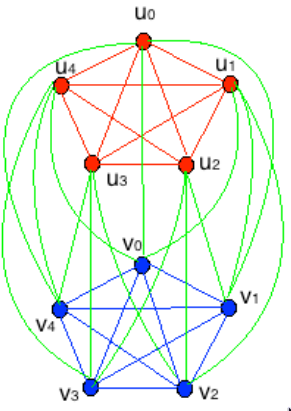
\includegraphics[width=0.3\linewidth]{images/WebCom.png}
    \caption{Esempio Web-Community con un solo nodo}
    \label{fig:wcexample}
\end{figure}

Se si osserva bene, comunque scegliamo un nodo $x$, l'\textit{unico} taglio minimo è del tipo $(\{x\}, V - \{x\})$, di dimensione 7. Infatti, se aggiungessimo un qualsiasi nodo insieme ad $x$ otterremmo un taglio di dimensione strettamente maggiore di 7.

Per esempio $12 = |(\{ u_0, u_1 \}, V - \{ u_0, u_1 \} )| >  |(\{ u_0 \}, V - \{ u_0 \} )| = 7$.

Se ci riveriamo alla definizione di cut-cumminity, non ha molto senso dire che il solo nodo $u_0$ compone una comunità, per questo è necessario dare una nuova definizione di comunità.

\subsection{Web-community}

Una web-community è un sottoinsieme dei nodi di un grafo, ciascuno dei quali ha più vicini fra i nodi del sottoinsieme che fra quelli esterni ad esso.

\begin{definizione}[Strong Web-community]
    Dato un grafo $G = (V, E)$, il sottoinsieme $C \subset V$ è una \textbf{strong web-community} se $C \neq \emptyset$ e
    \[
    \forall u \in C: |N(u) \cap C| > |N(u) \setminus C| = |N(u) \cap (V - C)|
    \]
    Alternativamente è comodo guardare alla precedente proprietà come il fatto che almeno la metà dei vicini di $u$ è all'interno di $C$.
    \[|N(u)| =  |N(u) \cap C| + |N(u) \setminus C| \implies  |N(u) \setminus C| = |N(u)| - |N(u) \cap C|\]
    Quindi, 
    \begin{align*}
        &\quad\quad\quad |N(u) \cap C| > |N(u) \setminus C| \\ 
        &\iff |N(u) \cap C| > |N(u)| - |N(u) \cap C| \\
        &\iff 2|N(u) \cap C| > |N(u)|\\ 
        &\iff \frac{|N(u) \cap C|}{|N(u)|} > \frac{1}{2}
    \end{align*}
\end{definizione}

\begin{definizione}[Weak Web-community]
    Dato un grafo $G = (V, E)$, il sottoinsieme $C \subset V$ è una \textbf{weak web-community} se $C \neq \emptyset$ e
    \[
    \forall u \in C: |N(u) \cap C| \geq |N(u) \setminus C| = |N(u) \cap (V - C)|
    \]
    Alternativamente è comodo guardare alla precedente proprietà come il fatto che almeno la metà dei vicini di $u$ è all'interno di $C$.
    \[|N(u)| =  |N(u) \cap C| + |N(u) \setminus C| \implies  |N(u) \setminus C| = |N(u)| - |N(u) \cap C|\]
    Quindi, 
    \begin{align*}
        &\quad\quad\quad |N(u) \cap C| \geq |N(u) \setminus C| \\ 
        &\iff |N(u) \cap C| \geq |N(u)| - |N(u) \cap C| \\
        &\iff 2|N(u) \cap C| \geq |N(u)|\\ 
        &\iff \frac{|N(u) \cap C|}{|N(u)|} \geq \frac{1}{2}
    \end{align*}
\end{definizione}

Queste definizioni possono essere generalizzate, richiedendo che:
\[
\frac{|N(u) \cap C|}{|N(u)|} > \alpha\ (\geq \alpha) \text{, per qualche costante } \alpha \in [0, 1]
\]

\newpage
\subsection{Relazione tra Cut e Web-communities}

\begin{teorema}[Relazione tra Cut e Web-communities]
    Sia $G = (V, E)$ un grafo; se $C \subset V$ è una cut-community per $G$ tale che $|C| > 1$. Allora, $C$ è una weak web-community per $G$.
\end{teorema}

\begin{proof}
    Supponiamo per assurdo che $C$ non sia una weak web-community. Allora, esiste un nodo $u \in C$ tale che $|N(u) \cap C| < |N(u) \setminus C|$. Poiché $|C| > 1$, allora esiste in $C$ un nodo $v$ distinto da $u$: ossia, $C \setminus \{u\} \neq \emptyset$.
    Inoltre
    \begin{align*}
        \underbrace{\vert (C \setminus \lbrace u \rbrace , (V \setminus C) \cup \lbrace u \rbrace ) \vert}_{\text{taglio indotto da} C' = C \setminus\{u\}}
        &= \vert (C, V \setminus C) \vert + \underbrace{\vert N(u) \cap C \vert - \vert N(u) \setminus C \vert}_{< 1 \text{, per ipotesi, } |N(u) \cap C| < |N(u) \setminus C|}\\
        &< \vert (C, V \setminus C) \vert
    \end{align*}
    Ponendo $C' = C \setminus \{u\}$ abbiamo trovato che il taglio indotto da $C'$ è \textbf{minore} del taglio indotto da $C$, e questo è assurdo in quanto essendo $C$ per ipotesi una cut-community deve essere vero che $(C, V \setminus C)$ è un taglio minimo di $G$. Perciò necessariamente è falsa l'ipotesi che $C$ non sia una weak web-community.
\end{proof}

Anche se esiste un algoritmo polinomiale che decide se un grafo è partizionabile in cut-community, non ne conosciamo uno che decida in tempo polinomiale se un grafo è partizionabile in web-communities.

Infatti, sappiamo trovare due cut-communities $C$, $V \setminus C$ che generino un taglio minimo, ma non sappiamo garantire che $|C| > 1$ e $|V \setminus C| > 1$. Infatti, osservando la \autoref{fig:wcexample}, $C = \{u_0\}$ è una cut-community, ma non è una web-community in quanto $u_0$ ha, ovviamente, più vicini in $V \setminus C$ che in $C$.

In realtà, non solo non conosciamo un algoritmo che possa farlo in tempo polinomiale, ma è possibile dimostrare che tale problema è \textbf{NP-completo}.

\subsection{Strong Web-Communities Partitiong (SWCP)}

Definiamo ora il problema decisionale \textbf{Strong Web-Communities Partitioning (SWCP)}. Dato un grafo $G = (V, E)$, decidere se esiste un sottoinsieme (proprio e non vuoto) $C$ di $V$ tale che $C$ e $V \setminus C$ sono due strong web-communities.

\begin{lemma}\label{lemma:swcp}
    Se $G=(V, E)$ è partizionabile in due strong web-communities e esistono $x, y, z \in V$ tali che $N(x) = \{y, z\}$ (ossia $x$ ha grado 2 in $G$), \textit{allora} per ogni $C \subset V$ tale che $C$ e $V \setminus C$ sono entrmabi due strong web-communities e i tre vertici $x, y, z \in C$ oppure $x, y, z \in V \setminus C$.
\end{lemma}
    In altre parole, Il lemma afferma che, in questa situazione, non è possibile che $y$ e $z$ si trovino in due community diverse: se il grafo è davvero partizionabile in due strong web-communities, allora i tre nodi $x,y,z$ devono stare tutti e tre nella stessa parte (tutti in $C$ oppure in $V \setminus C$.
\begin{proof}
    Sia $C \subset V$ tale che $C$ e $V \setminus C = \overline{C}$ sono due strong web-communities. Senza perdita di generalità, assumiamo che $x \in C$.
    \begin{itemize}
        \item Per assurdo, supponiamo che $y, z \in \overline{C}$, allora 
        \[
        |N(x) \cap C| = 0 < |N(x) \cap \overline{C}| = 2
        \]
        Per la definizione di strong web-community, ogni nodo appartenente a $C$ deve avere più connessioni dentro $C$ che fuori. Ma qui $x$ ha 0 dentro e 2 fuori, quindi $C$ non può essere una strong web-community.
        \item Per assurdo, supponiamo che $y \in C$ e $z \in \overline{C}$, allora
        \[
        |N(x) \cap C| = 1 = |N(x) \cap \overline{C}|
        \]
        La condizione di strong web-community richiede una disuguaglianza stretta (più collegamenti interni che esterni). Quindi anche qui la condizione è violata.
        \item Se invece $x \in V \setminus C$ e uno dei vicini fosse in $C$, si avrebbe lo stesso ragionamento inverso (stessi casi di sopra).
    \end{itemize}
    In conclusione, in tutti i casi verrebbe contraddetta l'ipotesi che $C$ e $V \setminus C$ sono due strong web-communities.
\end{proof}

\begin{teorema}
    SWCP è NP-completo.
\end{teorema}

\begin{proof}
    Innanzitutto dobbiamo verificare che il problema è \textbf{NP}: un certificato è un sottoinsieme $C \subset V$, e verificare che $C$ e $V \setminus C$ sono strong web-communities richiede tempo polinomiale in $|G|$. Quindi il problema è \textbf{NP}. Dobbiamo ora dimostrarne la completezza, riducendo a 3SAT.

    Siano:
    \begin{itemize}
        \item $X = \{x_1, \dots, x_n\}$ l'insieme delle variabili,
        \item $f = c_1 \land c_2 \land \dots \land c_m$ con $c_j = l_1 \lor l_2 \lor l_3$, 
        \item $l_{jh} \in X$ oppure $\lnot l_{jh}$ per $j = 1, \dots, m$ e $h = 1, 2, 3$.
    \end{itemize}

    Costruiamo ora un grafo costituito da due nodi "specializzati" $T$ e $F$ che potranno appartenere alla stessa comunità $C$ se e soltanto se $C = V$ (e quindi $C$ non è una comunità, poiché non è contenuta propriamente in $V$).

    In altre parole, l'insieme dei nodi $V$ contiene i nodi $T$ e $F$, che rappresenteranno le assegnazioni \texttt{true} e \texttt{false}.
    Questi due nodi sono posizionati nel grafo in modo tale che essi dovranno necessariamente appartenere a due comunità differenti affinché $G$ sia partizionabile in due strong web-community

    Per ogni variabile $x_i \in X$ definiamo il \textbf{gadget variabile} nel seguente modo:
    \begin{itemize}
        \item Inseriamo in $V$ i nodi $x_i, \lnot x_i(w_i), y_i, z_i, t_i, f_i$,
        \item Inseriamo in $E$ gli archi $(x_i,y_i), (x_i,z_i), (y_i,t_i), (t_i,T), (\lnot x_i, z_i), (\lnot x_i, y_i), (z_i, f_i), (f_i, F)$,
        \item Infine, inseriamo tanti nodi senza nome, collegati a $x_i$ e $\lnot x_i$ quante sono le clausole che contengono la variabile $x_i$ e $\lnot x_i$ più uno (come mostrato in \autoref{fig:gadget}).
    \end{itemize}
        \newpage
        \begin{figure}[ht!]
            \centering
            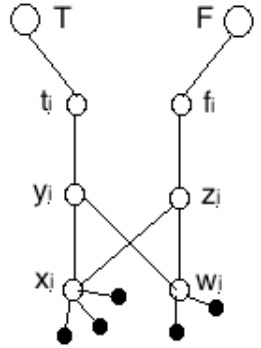
\includegraphics[width=0.2\linewidth]{images/gadgetxi.png}
            \caption{Gadget associato alla variabile $x_i$}
            \label{fig:gadget}
        \end{figure}
    Osserviamo che se $T$ ed $F$ appartengono a due comunità differenti, allora anche $x_i$ ed $\lnot x_i$ apparterranno a due comunità differenti. Infatti, senza perdita di generalità poniamo $T \in C$ e $F \in \overline{C} = V \setminus C$:
    poiché $t_i$ e $f_i$ hanno entrambi grado 2, per il \autoref{lemma:swcp} deve necessariamente essere vero che $t_i, y_i \in C$ e $f_i, z_i \in \overline{C}$. 

    Poiché $y_i$ ha grado 3, allora almeno uno tra $x_i$ e $\lnot x_i$ deve appartene a $C$.
    Stessa cosa per $z_i$, poiché ha grado 3 allora almeno uno tra $x_i$ e $\lnot x_i$ deve appartene a $\overline{C}$.

    Poiché $y_i$ e $z_i$ non devono poter essere raggiungibili (altrimenti apparterrebbero alla stessa comunità), allora possiamo dire che o $x_i$ appartiene e $C$ e $\lnot x_i$ a $\overline{C}$, oppure viceversa.

    Infine, per le osservazioni fatte sopra, anche ciascun nodo senza nome deve essere contenuto nella stessa comunità che contiene il padre.

    Continuando, per ogni clausola $c_j$ di $f$, definiamo un \textbf{gadget clausola} come segue:
    \begin{enumerate}
        \item Inseriamo in $V$ un nodo $c_j$ e un nodo per ognuno dei suoi letterali $l_{j1}, l_{j2}, l_{j3}$.
        \item In $E$ inseriamo gli archi da $c_j$ verso $l_{j1}, l_{j2}, l_{j3}$, e dai nodi $l_{j1}, l_{j2}, l_{j3}$ verso il nodo $T$.
        \item Infine, aggiungiamo in $E$ un arco da $c_j$ verso ognuno dei letterali che lo compongono: se in $c_j = x_1 \lor \lnot x_2 \lor x_3$ (\autoref{fig:ex_clausola}) allora inseriamo gli archi $(c_j, x_1), (c_j, \lnot x_2), (c_j, x_3)$.
    \end{enumerate}

    \begin{figure}
        \centering
        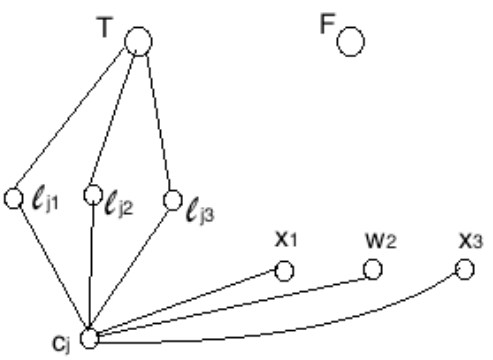
\includegraphics[width=0.3\linewidth]{images/ex_clausola.png}
        \caption{Clausola $c_j$}
        \label{fig:ex_clausola}
    \end{figure}

     Notiamo che sempre per il \autoref{lemma:swcp}, dato che $l_{j1},l_{j2},l_{j3}$ hanno tutti grado 2, allora se $G$ è partizionabile in due strong web-community, certamente sia $l_{j1},l_{j2},l_{j3}$ che $c_j$ devono essere nella stessa comunità a cui appartiene $T$.

     Dalla costruzione appena fatta emerge che quindi $c_j$ deve appartenere alla stessa comunità a cui appartiene $T$, e per rendere ciò possibile \text{almeno} uno dei letterali che lo compongono deve appartenere alla stessa comunità. Nell'esempio nella \autoref{fig:ex_clausola}, almeno uno tra $x_1, \lnot x_2, x_3$ deve essere contenuto in $C$, altrimenti $c_j$ avrebbe tanti vicini in $C$ quanti in $V \setminus C$.

    \begin{figure}[ht!]
        \centering
        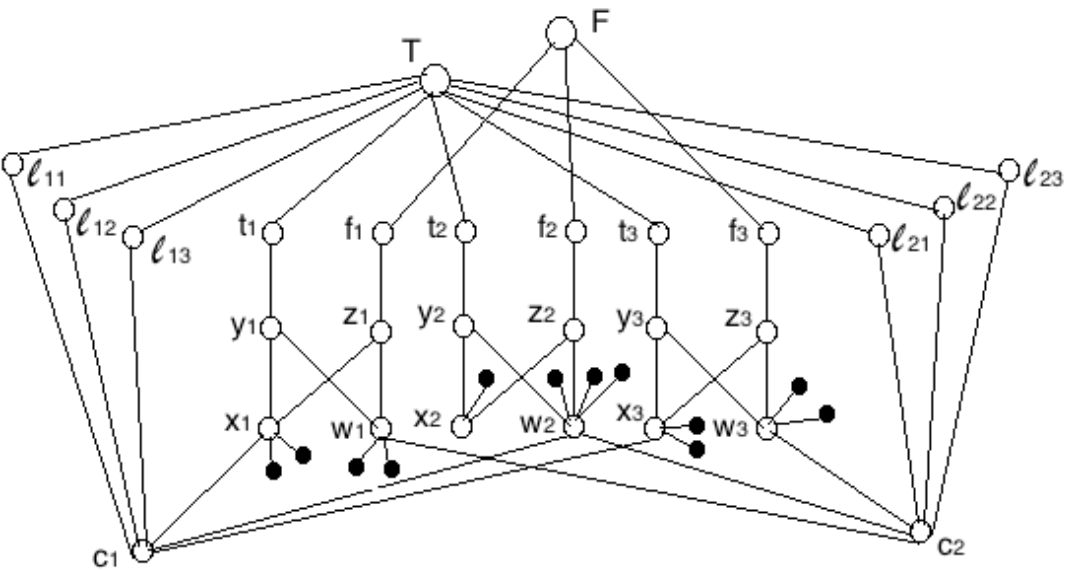
\includegraphics[width=0.5\linewidth]{images/funzione_completa.png}
        \caption{
            $f(x_1, x_2, x_3) = c_1 \land c_2 = (x_1 \lor \lnot x_2 \lor \lnot x_3) \land (\lnot x_1 \lor \lnot x_2 \lor \lnot x_3)$
            }
    \end{figure}

    Iniziamo col dimostrare che $T$ ed $F$ devono necessariamente appartenere a due comunità differenti, e questo verrà dimostrato dimostrando che se $T$ ed $F$ appartengono alla stessa comunità $C$ allora $C \equiv V$
    \[
    T, F \in C \Leftrightarrow C \equiv V
    \]
    Iniziamo con l'osservare che se $T,F$ appartengono alla stessa comunità $C$ allora anche i nodi $y_i$ e $z_i$ appartengono a $C$, per ogni $i = 1, 2, \dots, n$.
    
    Consideriamo il letterale $x_i$ che è contenuto in $k$ clausole del tipo $c_j$.
    Poiché ognuna di queste clausole sono per costruzione nella stessa comunità di $T$ (e quindi in $C$) e poiché $x_i$ ha altri due suoi vicini $y_i, z_i$ in $C$, risulterà che più della metà dei suoi vicini sono in $C$. Infatti risulta che $x_i$ ha esattamente $k+2$ vicini in $C$ più altri $k+1$ nodi senza nome.
    Perciò, dovunque inseriamo qui $k+1$ nodi senza nome, per forza $x_i$ deve stare in $C$. Stesso ragionamento per $\lnot x_i$.
    
    \begin{figure}[ht!]
        \centering
        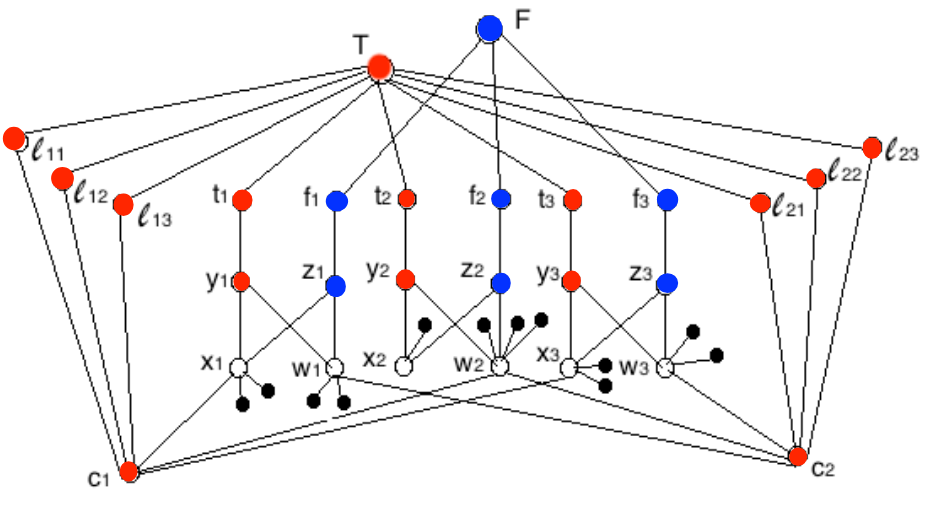
\includegraphics[width=0.5\linewidth]{images/funzione_completa_col.png}
        \caption{}
        \label{fig:funzione_completa_col}
    \end{figure}

    Per comprendere meglio il concetto, osserviamo la \autoref{fig:funzione_completa_col}. Se $T$ e $F$ sono due diverse comunità, allora, per ogni $c_j$ i nodi $c_j, l_{j1}, l_{j2}, l_{j3}$ sono nella stessa comunità di $T$ (nodi in rosso). Per ogni variabile $x_i$, i nodi $t_i$ e $y_i$ sono con $T$ (rossi) e i nodi $f_i$ e $z_i$ sono con $F$ (blu).
    Allora, dobbiamo "colorare" i nodi $x_i$ e $\lnot x_i (w_i)$ per ogni variabile $x_i$, in modo che l'insieme dei nodi rossi e l'insieme dei nodi blu siano strong web-communities.

    Riassumendo, $G$ è partizionabile in due strong web-communities $C$ e $V \setminus C$ se e soltanto se $T$ e $F$ \textbf{non} sono entrambi in $C$ e non sono entrambi in $V \setminus C$, ovvero appartengono a comunità diverse.

    Quindi, affinché $T \in C$ e $F \in V \setminus C$, devono valere le seguenti due proprietà:
    \begin{enumerate}
        \item Per ogni variabile $x_i \in X$, \textbf{esattamente uno dei nodi $x_i$ e $\lnot x_i$ deve essere contenuto in $C$ e esattamente uno dei nodi $x_i$ e $\lnot x_i$ deve essere contenuto in $V \setminus C$}. 
        
        Allora, ogni partizione in $G$ in due strong web communities corrisponde ad una assegnazione di verità $a$ per $X$ che soddisfa $f$. 

        \[
            a(x_i) = 
            \begin{cases}
                \texttt{true}& if\  x_i \in C\\
                \texttt{false} & if\ x_i \in V \setminus C
            \end{cases}
        \]
        dove $C$ è la comunità a cui appartiene $T$.
        
        Viceversa, se esiste un'assegnazione $a: X \rightarrow \lbrace \texttt{true}, \texttt{false} \rbrace$ che soddisfa $f$, allora è possibile ricavare una partizione di $G$ in due web-communities.

        \item Per ogni clausola $c_j$, il nodo $c_j$ \textbf{deve} appartenere a $C$ (che contiene $T$), e perché questo sia possibile \textbf{è necessario che almeno uno dei nodi nei gadget variabile collegato a $c_j$ sia contenuto in $C$, ossia, uno dei nodi corrispondenti a un letterale nella clausola $c_j$ deve essere contenuto in $C$}.

        Innanzitutto poniamo $T$ in $C$ ed $F$ in $V \setminus C$. Dopodiché, dato che $a$ soddisfa $f$, allora inseriamo in $C$ tutti i nodi clausola $c_j$ e i rispettivi $l_{j1}, l_{j2}, l_{j3}$. Infine, per ogni $i$, inseriamo in $C$ i seguenti nodi:
        \begin{itemize}
            \item  se $a(x_i) = \texttt{true}$, inseriamo $x_i$, i suoi nodi senza nomi, e i nodi $y_i, t_i$.
            \item se $a(x_i) = \texttt{false}$, inseriamo $\overline{x_i}$, i suoi nodi senza nomi, e i nodi $y_i, t_i$.
        \end{itemize}
    \end{enumerate}
        
    Le due comunità risultanti saranno due cut-communites.
\end{proof}

\newpage

\section{Partizionare un grafo in comunità:
approccio euristico}

In questa parte verranno mostrate due famiglie approcci che dal punto di vista euristico riescono a partizionare un grafo in comunità accettabili, ovvero in gruppi di nodi abbastanza coesi tra di loro.

Più precisamente i due metodi si dividono in:
\begin{itemize}
    \item \textbf{Metodi partitivi}, in cui si parte considerando l'intero grafo come unica grande comunità, e la si inizia a disconnettere (rimuovendo archi) finché non si otterranno due comunità distinte e coese. Se si desidera ottenere una \textbf{granularità} maggiore basta iterare il metodo sui sotto grafi ottenuti.
    \item \textbf{Metodi agglomerativi}, in cui si parte considerando ogni singolo nodo una comunità, e man mano si aggiungono gli archi del grafo finché non si otterranno un numero di comunità desiderato con un livello di coesione accettabile.
\end{itemize}

\subsection{Betwenness di un Arco}

Vediamo ora un particolare criterio per rimuovere gli archi in un metodo partitivo. In particolare, il criterio che andremo a vedere si basa sul concetto di \textbf{betwenness di un arco}, che a sua volta si basa sui concetti di bridge e local bridge. Ricordiamo che un bridge (per definizione), connette due regioni del grafo che altrimenti risulterebbero non connesse. Mentre un bridge, connette due regioni che, senza di esso, sarebbero connesse in modo meno efficiente. Possiamo quindi dire che bridges e local bridges connettono regioni che, senza di loro, avrebbero difficoltà ad interagire. Inoltre, sappiamo che questi arco sono weak ties, quindi gli archi che rimangono dopo la loro rimozione sono gli strong ties - quelli delle relazioni forti.

Quindi l'idea alla base di questo criterio è la seguente: rimuovendo bridges e local bridges il grafo viene partizionato in componenti che bene pososno essere considerate comunità.

Consideriamo la rete in \autoref{fig:controesempio_weak_strong}. Non è presente nessun local bridge, ma è facile osservare che esitono due comunità (cerchiate in rosso).

\begin{figure}
    \centering
    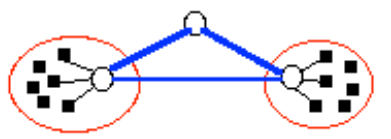
\includegraphics[width=0.5\linewidth]{images/BTcontroesempio.png}
    \caption{Controesempio weak/strong ties}
    \label{fig:controesempio_weak_strong}
\end{figure}

Al fine di definire il metodo partitivo, è necessario definire il concetto di betwenness di un arco. Essa è basato sulla nozione di traffico (o flusso) di informazioni che passa attraverso gli archi.

Possiamo considerare come "nuovi archi ponte" tutti quegli archi attraverso i quali passa una grande quantità di flusso, e che se rimossi rendono più difficile la comunicazione tra due comunità.

Secondo questo criterio possiamo rimuovere gli archi sui quali passa maggior flusso, finché non otterremo un partizionamento accettabile della rete.


Sia $G=(V, E)$ non orientato.
\begin{definizione}
    Definiamo con $\sigma_{st}(u,v)$ il numero di \textbf{shortest-paths} (\textbf{camminimi minimi}) $\pi^\star(s,t)$  tra $s$ e $t$ che passano per l'arco $(u,v)$.
    \[
    \sigma_{st} = |\{\pi^\star(s,t)\}|
    \]
\end{definizione}

\begin{definizione}[Betweeness Relativa]
    Definiamo poi con $b_{st}(u,v)$ la \textbf{betweennes relativa} all'arco $(u,v)$ \textbf{rispetto alla coppia} $s,t$ come la \textbf{frazione} di shortest path $\pi^\star(s,t)$ che passano per l'arco $(u,v)$.
    \[
        b_{st}(u,v) = \frac{\sigma_{st}(u,v)}{\sigma_{st}}
    \]
\end{definizione}

\begin{definizione}[Betweeness Totale]
    Definiamo la \textbf{betweenness} $b(u,v)$ di un arco $(u,v)$ come la \textbf{semi-somma} di tutte le betweenness relative $b_{st}(u,v)$, per ogni coppia di nodi $s,t$
    \[
    b(u,v) = \frac{1}{2} \sum_{(s,t) \in \binom{V}{2}} b_{st}(u,v)
    \]
Notare che il fattore $1/2$ è necessario per evitare di contare le ripetizioni, del tipo $b_{st}(u,v)$ e $b_{ts}(u,v)$.
\end{definizione}

Analogamente alla \textbf{edge-betweenness} si può definire una \textbf{node-betweenness}, seguendo la stessa definizione.

\subsection{Metodo di Girvan-Newman}

Il metodo di Girvan-Newman è un metodo partitivo che si basa sulla betweenness. Si inizia considerando l'intero grafo coem un'unica grande comunità, poi si calcola l'arco di betweenness massima e si rimuove: se il grafo residuo è non connesso allroa è stata ottenuta una prima partzione in comunità. Il procedimento viene poi iterato calcolando gli archi di betweenness massima nel grafo rimanente e rimuovendoli. Il procedimento ha termine quando si è ottenuto un livello di granularità ritenuto adeguato.

Lo schema dell'algoritmo per il calcolo delle betweenness degli archi è il seguente:

Per ogni $s \in V$, si eseguono i seguenti tre passi:
\begin{enumerate}
    \item Calcola il sottografo $T(s)$ degli shortest path uscenti da $s$ mediante una BFS.
    \item Mediante una visita \textbf{top-down} di $T(s)$, per ogni nodo $V \in V$ calcola $\sigma_{sv}$ (numero di shortest path da $s$ a $v$).
    \item Mediante una visita \textbf{bottom-up} di $T(s)$, e usando quanto calcolato al punto (2), per ogni $(u, v) \in T(s)$ calcola 
    \[
        b_s(u,v) = \sum_{t \in V \setminus \{s\}} b_{st}(u, v)    
    \]
\end{enumerate}
Infine, per ogni arco $(u,v) \in E$, si calcola 
\[
    b(u,v) = \frac{1}{2} \sum_{(s,t) \in \binom{V}{2}} b_{st}(u,v)
\]

Vediamo meglio nel dettaglio come funzionano le fasi (1), (2) e (3).

\subsubsection{Fase 1}
Per calcolare $T(s)$ basta effettuare una visita in ampiezza \textbf{BFS} opportunamente modificata.

Definiamo con $L_h$ l'insieme di tutti i nodi a distanza $h$ dalla sorgente $s$.
Diremo che un nodo $v$ si trova al \textbf{livello} $h$ se $v \in L_h$.

Se un nodo $v$ si trova al livello $h$, allora certamente \textbf{tutti} i cammini minimi da $s$ a $v$ termineranno con archi che partono da $L_{h-1}$.
Perciò, tutti gli archi $(u,v)$ con $u \in L_{h-1}$ e $v \in L_h$ faranno parte di $T(s)$.

Perciò possiamo calcolare $T(s)$ nella seguente maniera (\autoref{fig:fase1}):

\begin{enumerate}
    \item Poniamo inizialmente $L_0 = \lbrace s \rbrace$ e $T(s) = \emptyset$.
    \item Per ogni $h \geq 0$ calcoliamo $L_{h+1}$ come tutti quei nodi \textbf{fuori} $L_0 \cup L_1 \cup \dots \cup L_h$ tali che hanno almeno un vicino in $v \in L_h$, ovvero come
    \[
    L_{h+1} \equiv \{ v \in V \setminus (L_0 \cup L_1 \cup \dots \cup L_h)\ |\ \exists u \in L_h : (u,v) \in E  \}
    \]
    \item Calcolato $L_{h+1}$ poniamo $T(s)$ come 
    \[
    T(s) = T(s) \cup \{ (u,v) \in E\ |\ u \in L_h \land v \in L_{h+1} \}
    \]
\end{enumerate}
    \begin{figure}[ht!]
        \centering
        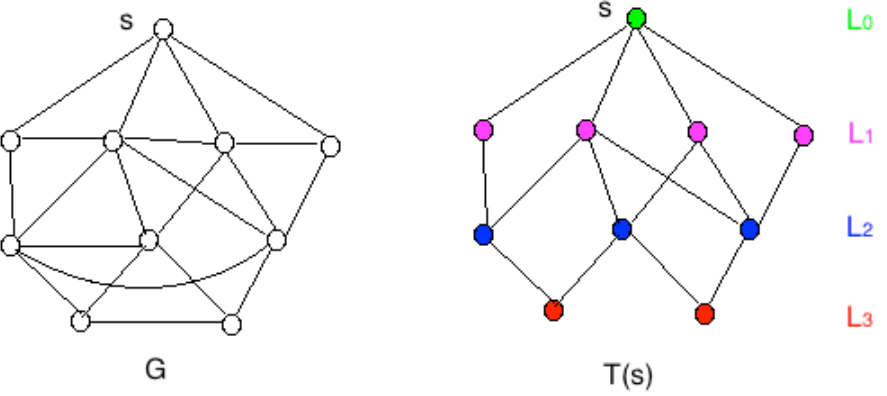
\includegraphics[width=1\linewidth]{images/fase1GN.png}
        \caption{Costruzione sottografo cammini minimi}
        \label{fig:fase1}
    \end{figure}

\newpage
\subsubsection{Fase 2}

Calcolato $T(s)$, possiamo sfruttarlo per calcolare, per ogni $v \in V$, la quantità $\sigma_{sv}$, ovvero il numero di cammini minimi che vanno da $s$ a $v$.

In altre parole, il numero numero di shortes paths dalla radice $s$ a un nodo $v \in L_h$ è pari alla somma dei numero dei percorsi da $s$ a un qualunque "padre" di $v$.

Iniziamo osservando che per ogni nodo $v$ nel livello 1, il numero di cammini minimi sarà pari ad 1 (perché $v$ è diretto vicino di $s$).

Invece al livello 2, il numero di cammini minimi di un generico nodo $v \in L_2$ è pari alla somma di tutti i $\sigma_{su}$, tali che esiste $(u,v)$ con $u \in L_1$. Più in generale, per ogni $v \in L_h$, possiamo calcolare $\sigma_{sv}$ con la seguente formula ricorsiva
\[
	\sigma_{sv} =\begin{cases}
    1  & \text{if } h = 1\\
	\sum\limits_{(u,v) \in E\ |\ u \in L_{h-1}} \sigma_{su}  & \text{if }h > 1
	\end{cases} 
\]

\begin{figure}[ht!]
    \centering
    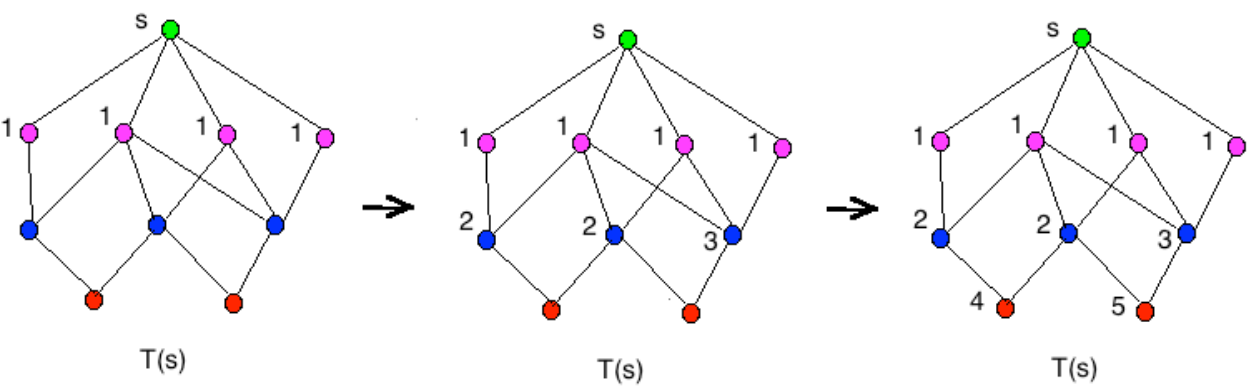
\includegraphics[width=0.8\linewidth]{images/fase_2.png}
    \caption{Calcolo dei cammini minimi in $T(s)$}
    \label{fig:fase2}
\end{figure}

\subsubsection{Fase 3}

Nella terza fase dobbiamo calcolare per ogni arco $(u,v) \in T(s)$ la quantità di flusso che ci passa sopra rispetto a $s$, ovvero 
\[
    b_s(u,v) = \sum_{t \in V \setminus \{ s \}} b_{st}(u,v)
\]
Per fare ciò in questo caso faremo una visita "bottom-up" di $T(s)$.

Sia $d$ il numero di livelli in $T(s)$, e consideriamo un arco $(y,x)$ con $y \in L_{d-1}$ e $x \in L_d$. 

Osserviamo che tutti gli shortest path che partono da $s$ e passano attraverso l'arco $(y,x)$ sono tutti shortest path che terminano in $x$.

Perciò il flusso che passa su $(y,x)$ rispetto a $s$ sarà pari al rapporto tra il numero di shortest path che vanno da $s$ a $y$ (ovvero $\sigma_{sy}$) e il numero complessivo di shortest path che vanno da $s$ ad $x$ (ovvero $\sigma_{sx}$).
\[
b_s(y,x) = \sum_{t \in V \setminus \{ s \}} b_{st}(y,x) = b_{sx}(y,x) = \frac{\sigma_{sx}(y,x)}{\sigma_{sx}} = \frac{\sigma_{sy}}{\sigma_{sx}}
\]
Analogamente possiamo applicare questo ragionamento per tutti gli archi che collegano nodi dell'ultimo livello, come mostrato in \autoref{fig:fase3_a}.

\newpage

\begin{figure}[ht!]
    \centering
    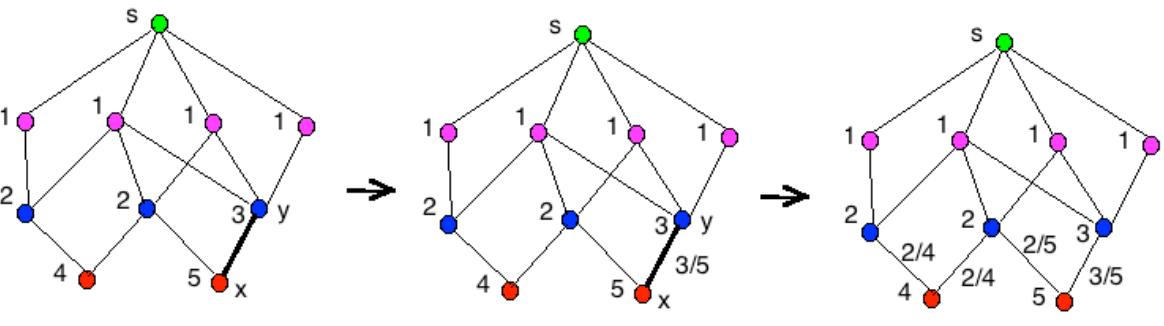
\includegraphics[width=0.8\linewidth]{images/fase3_a.png}
    \caption{Calcolo di $b_s(y,x)$}
    \label{fig:fase3_a}
\end{figure}

Adesso, saliamo di un livello, e consideriamo gli archi che entrano nel livello $L_{d-1}$.

Rifacendoci alla \autoref{fig:fase3_b}, consideriamo l'arco $(z, y)$, con $z \in L_{d-2}$ e $y \in L_{d-1}$.

\begin{figure}[ht!]
    \centering
    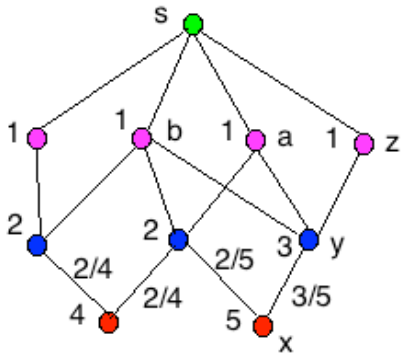
\includegraphics[width=0.3\linewidth]{images/fase3_b.png}
    \caption{Immagine in esempio}
    \label{fig:fase3_b}
\end{figure}

Osserviamo che tra tutti i cammini minimi che passano per l'arco $(z, y)$, una parte saranno cammini che termineranno in $y$, e una parte saranno cammini minimi che andranno ai nodi di livello inferiore.

Perciò la frazione di shortest path che, partendo da $s$, passano per $(z, y)$ è pari alla somma dei seguenti fattori:
\begin{itemize}
    \item La frazione degli shortest path da $s$ ad $y$, ovvero $\frac{\sigma_{sz}}{\sigma_{sy}}$. 
    \item Per ogni \textbf{diretto discendente} $x$ di $y$, una frazione $\frac{\sigma_{sz}}{\sigma_{sy}}$ della frazione di shortest path da $s$ ad $x$ che passano per l'arco $(y,x)$, ovvero 
    \[
    \frac{\sigma_{sz}}{\sigma_{sy}} \cdot \frac{\sigma_{sy}}{\sigma_{sx}} = \frac{\sigma_{sz}}{\sigma_{sx}}
    \]
\end{itemize}


Quindi, rifacendoci all'esempio, avremo che 
\[
b_s(z,y) = \frac{\sigma_{sz}}{\sigma_{sy}} + \frac{\sigma_{sz}}{\sigma_{sy}} \cdot \frac{\sigma_{sy}}{\sigma_{sx}} = \frac{1}{3} + \frac{1}{3}\cdot\frac{3}{5} = \frac{8}{15}
\]
Così facendo abbiamo definito un metodo "bottom-up" per il calcolo tutti i valori $b_s(u,v)$.

Infine, dopo l'esecuzione di queste 3 fasi, calcoliamo la betweenness finale come:
\[
    b(u,v) = \frac{1}{2} \sum_{s \in V} b_s(u,v)
\]

Notiamo che questa procedura permette di calcolare la betweennes degli archi in tempo \textbf{polinomiale} nella grandezza della rete (e non esponenziale).

Infatti la (1) è una semplice visita in ampiezza del grafo (e si può calcolare in tempo $O(|V| + |E|)$), la (2) è un'ulteriore visita in ampiezza di $T(s)$ (e si può calcolare ancora in tempo $O(|V| + |E|)$), e infine la (3) è nuovamente una visita in ampiezza, partendo però dal livello più basso (ancora una volta $O(|V| + |E|)$).

Dato che bisogna iterare questo procedimento per ogni nodo del grafo, e dato che nel caso peggiore abbiamo grafi molto densi con $\Theta(n^2)$ archi, la complessità temporale dell'esecuzione di questo algoritmo per il calcolo delle betweennes sarà $O(nm) \in O(n^3)$.

\section{Rilassare il Modello}

Nel modello teorico originale delle reti sociali, le relazioni venivano considerate in modo dicotomico: gli archi potevano essere \textit{strong ties} o \textit{weak ties}, e alcuni potevano essere \textit{bridge edges}. Tuttavia, questo approccio è troppo rigido per le reti reali, dove raramente esistono veri \textit{bridge edges} e la forza delle relazioni non è classificabile in modo netto.

Per rendere il modello più realistico, si introduce quindi una \textbf{rete pesata}:
\[
G = (V, E, w) \text{ dove } w : E \rightarrow \mathbb{N}
\]
ossia $w(u,v)$ rappresenta numericamente la \textit{forza} del legame tra due nodi.

Il concetto di \textit{bridge edge} viene sostituito dal \textbf{neighborhood overlap (NO)}, che misura la frazione di amici in comune tra due nodi:
\[
NO(u,v) = \frac{|N(u) \cap N(v)|}{|N(u) \cup N(v) - {u,v}|}
\]
Un \textit{local bridge} ha dunque $NO(u,v) = 0$.

Poiché nel modello classico la Strong Triadic Closure Property garantisce che i local bridge siano weak ties, ci si chiede se una relazione simile tra forza del legame e ruolo strutturale esista anche nel modello pesato.

A supporto di questa idea vi sono i risultati empirici di \textbf{Onnela et al. (2007)}, che analizzarono una grande rete telefonica reale. Essi costruirono un grafo dai dati delle chiamate e procedettero a rimuovere gli archi:

\begin{enumerate}
    \item prima rimuovendo quelli con \textbf{peso alto}, osservando che la rete rimaneva connessa a lungo;
    \item poi rimuovendo quelli con \textbf{peso basso} osservando la rete si disconnetteva rapidamente.
\end{enumerate}

Questi risultati suggeriscono che gli archi con peso basso svolgono un ruolo cruciale nel collegare comunità diverse e quindi hanno \textbf{basso neighborhood overlap}, analogamente ai weak ties del modello classico.

In sintesi, anche nel modello rilassato sembra esistere una correlazione empirica tra \textbf{bassa forza del legame} (peso) e \textbf{basso neighborhood overlap}, analoga alla relazione tra weak ties e local bridges.

\section{Conclusioni}

Ricapitolando, una rete sociale può essere vista come un insieme di gruppi 
densamente connessi tramite relazioni forti, mentre tali gruppi sono a loro volta 
collegati tra loro attraverso relazioni deboli.

Dal punto di vista sociale, l'appartenenza ad un gruppo porta numerosi vantaggi: 
più un individuo è ben inserito all'interno del proprio gruppo --- ovvero più gode 
della fiducia dei suoi vicini --- maggiori benefici ottiene. Contrariamente, 
l'esperimento di Granovetter mostra che è spesso altrettanto utile mantenere 
connessioni con individui appartenenti ad altri gruppi, poiché questo permette 
di accedere a nuove e potenzialmente vantaggiose fonti di informazione.

Queste osservazioni suggeriscono che i vantaggi di un nodo non dipendono solo 
dalla sua appartenenza ad una comunità, ma anche dalla sua posizione nella rete 
e dal grado di integrazione nel proprio gruppo. Per formalizzare questa idea 
introduciamo il concetto di \textbf{embeddedness} di un arco $(u,v)$, definito come 
la quantità di vicinato condiviso tra i due nodi:
\[
\text{Emb}(u,v) = |N(u) \cap N(v)|.
\]
Si osserva che un \textit{local bridge} è un arco con embeddedness pari a $0$.

Una embeddedness elevata indica che i due estremi dell'arco sono ben integrati 
nella stessa comunità. Analogamente, un nodo che presenta molti archi con alta 
embeddedness è un nodo fortemente inserito nel proprio gruppo.

Nell'esempio precedente, il nodo \texttt{A} risulta ben integrato nella sua 
comunità, in quanto occupa una posizione centrale: tutti i suoi archi hanno 
embeddedness elevata. Al contrario, il nodo \texttt{B} si trova in una posizione 
marginale, avendo pochi archi con embeddedness alta.


